

\chapter{Evaluation} \label{Chapter6}

%; including, but not limited to, machine type advertised, publicly open ports, running processes etc.
This chapter focuses on providing an evaluation of the implemented cyber incident monitoring system, as well describing the design and conducting of experiments as part of the proposal for adaptive honeypot design.

\textit{Section \ref{DesignOfExperiments}} provides an in-depth explanation of how the experiments were designed for evaluating the impact of attractiveness honeypot characteristics on the number of attacks received.

\textit{Section \ref{ConductingExperiments}} discusses how the experiments were conducted and their limited findings, detailing the nature of numerous setbacks that occurred and how these were dealt with. An explanation for the early conclusion of these experiments is also provided.

\textit{Section \ref{DiscussionOfEvaluation}} discusses the limited findings of the experiments as well as a qualitative evaluation of the cyber incident monitoring solution produced.

Finally, \textit{Section \ref{SummaryOfChapter6}} provides some brief conclusions regarding the evaluation of the honeypot experiments.

\section{Design of Experiments \label{DesignOfExperiments}}
The conducting of experiments in this research is focused on the delivery of the second objective outlined in \textit{Section \ref{Objective2}}: To determine an improved design for effective, adaptive honeypots. It was decided that the measure of effectiveness in these experiments would be defined by how many attacks each honeypot received. From this, it would be possible to present findings and draw conclusions regarding the development of effective adaptive honeypots. 

The design of the experiments was influenced greatly by the time that remained to complete the entirety of the research: A period of just four weeks. A series of experiment iterations were devised to be run over the course of these 4 weeks. Table \ref{table:HoneypotExperimentsTable} describes the variables involved in each iteration, and the intended execution of these iterations with respect to time. 


\begin{table}[!h]
\begin{center}
\begin{tabular}{|*{17}{c|}}  % repeats {c|} 17 times
\hline
\multicolumn{1}{|c}{} & \multicolumn{4}{|c|}{\textbf{Vendor A}} & \multicolumn{4}{|c|}{\textbf{Vendor B}} & \multicolumn{4}{|c|}{\textbf{Vendor C}} & \multicolumn{4}{|c|}{\textbf{Control}} \\ \hline
\multicolumn{1}{|c}{} &
\multicolumn{4}{|c}{\textit{Week 1}} & \multicolumn{4}{|c}{\textit{Week 2}} & \multicolumn{4}{|c}{\textit{Week 3}} & \multicolumn{4}{|c|}{\textit{Week 4}} \\ \hline 
 & \textbf{LC} & \textbf{SA} & \textbf{DT} &  & \textbf{LC} &\textbf{SA} & \textbf{DT} &  &\textbf{LC} & \textbf{SA} & \textbf{DT} & & \textbf{LC} &\textbf{SA} & \textbf{DT} & \\ \hline
\textbf{HP1} & A & X & P &  & A &X & P &  &A & X & P & &A & X &P &  \\ \hline
\textbf{HP2} & B & Y & Q &  & B &Y & Q &  &B & Y & Q & &B & Y &Q &  \\ \hline
\textbf{...} & C & Z & R &  & C &Z & R &  &C & Z & R & &C & Z &R &  \\ \hline
\textbf{HPN} & D & W & S &  & D &W & S &  &D & W & S & &D & W &S &  \\ \hline
\textbf{Control} & * & * & * &  & * &* & * &  &* & * & * & &* & * &* &  \\ \hline
 \end{tabular}
\end{center}
 \caption[Planned Iterations of the Honeypot Experiments]{A set of planned experiment iterations in order to propose an optimal honeypot design. Three characteristics of the N Cowrie honeypots HP1, HP2 ... HPN are considered: The login credentials accepted (\textit{LC}), the services advertised to be running on the container (\textit{SA}), and the type of device advertised (\textit{DT}). For each week, only one characteristic of the router honeypot is varied: The device vendor, corresponding to columns \textit{Model A, Model B,} etc. Each variation of a Cowrie honeypot characteristic (\textit{LC, SA, DT}) should be in place for 2 days, with all 12 experiment iterations taking place over 4 weeks. There is one day allocated per 7-day week for setting up the experiments, represented by the empty column for each week. In each iteration there is a single \textit{Control} Cowrie honeypot used as an indication of baseline performance, and in \textit{Week 4} a \textit{Control} router honeypot is also employed for the same reason.}	
\label{table:HoneypotExperimentsTable}
\end{table}

An explanation of how this plan translates into the configuration of the research environment is explained in the following subsections.

\subsection{Router Honeypot Container}
As the gateway between the public internet and the Cowrie honeynet, it is obvious that the router container should aid an attacker in accessing the deployed system. Facilitating easy access to this container is likely to increase the chance of a successful venture into the Cowrie honeynet, enabling valuable data to be captured. Thus, it was important to configure the router container to be as attractive and open as possible to the targeted attackers, IoT botnets. 

The system had already been designed and implemented to facilitate exactly these requirements, and so the router container could easily provide:

\begin{itemize}
\item Remote access over either SSH or telnet from the public internet;
\item Authentication using a number of valid username-password combinations;
\item Root privileges inside the system;
\item A powerful OS and toolkits;
\item A network of nearby hosts to which an attack could be propagated;
\item An attractive device banner indicating a device type.
\end{itemize}

In order to gain some insights regarding honeypot design from the router container  and not just from the Cowrie honeypots, it was decided to vary a characteristic of the router container honeypot as part of the experiments: The device vendor advertised\footnote{In order to facilitate easy access to the Cowrie honeynet whilst also gaining some insights from allowing attackers to access the router container, the device vendor advertised in the SSH and telnet banners of the router honeypot was deemed to be a suitable and useful characteristic to measure. If this characteristic was found to impact upon the number of attacks received, it would give an indication of vendor awareness in IoT botnets.}. All other characteristics of the router container would be held constant, such that the same username-password credentials, services, toolkits, etc. would be available on this honeypot in all experiment iterations. 

% over a number of iterations of experiments, one characteristic of the router container would be varied: 


With reference to the experiment iterations plan in table \ref{table:HoneypotExperimentsTable}, the following experiments were designed for the measurement of the impact of device vendor on the number of attacks received:

\begin{itemize}
\item For each of \textit{Week 1}, \textit{Week 2} and \textit{Week 3} shown in the table, the router container would be configured to advertise a different brand of router to through SSH and telnet banners. Each banner will be left on the router container for 6 consecutive days of that week, with every other variable in the router honeypot environment being held constant.
\item In \textit{Week 4}, a \textit{Control} router container would be used: One which doesn't advertise any brand or model, but which simply uses the default 'Ubuntu 16.0.4 LTS' SSH and telnet banner with hostname \textit{router}. By having a control, it is possible to compare the results of the other three weeks against a baseline to determine whether or not it matters that a device is advertised as being from a particular vendor.
\end{itemize}

For the 3 device banners to be configured on this honeypot for \textit{Week 1}, \textit{Week 2} and \textit{Week 3}, it is desirable to base those device brands used in the banner configuration on real-world data. Masscan is a powerful asynchronous port scanner which was used by the researchers behind the IoTPot honeypot to capture device banners from devices on the public internet listening on the telnet 23/TCP port. \cite{IoTPot2016} The researchers used these banners to customise the honeypots to look like a real telnet-enabled device on the Internet. The effectiveness of this approach in their evaluation of IoT botnet behaviour motivated the decision to use Masscan to capture device banners in this research for use in the experiments. The most commonly occurring device vendor banners would be used as a basis for the experiments, since a more popular device vendor can be assumed to be more likely to be attacked than a less popular one.

%After the end of the first week, I will change the brand/model of the router advertised - e.g. Netgear, Cisco, etc. depending on the most common banners from the masscan data. I will repeat the same experiments as before for the cowrie honeynet however, in order to ensure that I can clearly attribute any trends to a particular variation in a single parameter.


\subsection{Cowrie Honeypot Containers}
In the Cowrie honeynet, there is substantially more scope for measuring the impact of varying honeypot characteristics since there are a greater number of honeypots available: As motivated in the formulation of the research objectives in \textit{Section \ref{BenefitsForUsingHoneynetForExperiments}}, a honeynet provides a solution to the accurate measurement of relative effectiveness of honeypots in the same environment, since the effects of time can be largely disregarded\footnote{Since all honeypots in the honeynet should be simultaneously exposed to the same environmental conditions, the effect of time variability in the experiments is minimised.}.
% * <rohiggin@tcd.ie> 2018-05-16T14:01:08.245Z:
% 
% > \textit{Section \ref{BenefitsOfUsingHoneynetsForExperiment}},
% Add correct Section, comes up as "??"
% 
% ^.

For each of the 4 weeks for which the experiments would be run, it was decided that 3 honeypot characteristics would be varied for a period of 2 days per week each. These characteristics are:


\begin{enumerate}
\item The login credentials accepted by the honeypot;
\item The services running on the honeypot's container ports\footnote{In the research conducted by Dowling \textit{et al.} in the implementation of a Zigbee honeypot, the generation of unencrypted network traffic was an interesting honeypot characteristic used in an attempt to attract the attention of attackers. \cite{Dowling2017} Measuring the impact that such a measure has on the number of attacks received by a honeypot was deemed a useful characteristic to measure.};
\item The type of device advertised by the honeypot.
\end{enumerate}

To illustrate how this translates into an experiment iteration, consider column \textit{LC} in \textit{Week 1} in table \textit{\ref{table:HoneypotExperimentsTable}} as an example.
\begin{itemize}
\item \textit{LC} corresponds to the variation of the \textit{login credentials} accepted by honeypots HP1, HP2, ... HPN over a 2-day period.
\item For each of honeypots HP1, HP2, ... HPN, the login credentials accepted should vary. Other variabls should be held constant\footnote{This means that if the \textit{login credentials} (\textit{LC}) are the characteristic being varied, both the \textit{services advertised} (\textit{SA}) and the \textit{device type} (\textit{DT}) should be held constant}.
\end{itemize}

It was decided that five Cowrie honeypots would be deployed in each experiment iteration, one of which would be the control honeypot. The presence of a control iteration is important, since it allows for definitive conclusions to be drawn as to whether or not the results obtained by customised honeypots have any impact on the number of attacks they receive. 

% Wikipedia definition of experiment control: designed to minimize the effects of variables other than the independent variable. This increases the reliability of the results, often through a comparison between control measurements and the other measurements.

 
%
%	SECTION 2: CONDUCTING EXPERIMENTS
%
 

 \section{Conducting Experiments} \label{ConductingExperiments}
The experiment iterations were planned to be conducted in the order in which they are specified in table \ref{table:HoneypotExperimentsTable}, starting with varying the login credentials of the Cowrie honeypots and the addition of a banner advertising a device manufacturer.


\subsection{Capturing Device Banners}
Masscan was used to scan the entire IPv4 address space for devices listening on ports 22/TCP (SSH) or 23/TCP (telnet) over the course of two days. The telnet and SSH banners of any device that responded were captured in log files. The IP addresses of these devices were also captured.

The banners were extracted from the log files into a new file, where they were counted using shell commands. In total, 71,149 banners were captured after scanning port 23/TCP (telnet) and 179,849 banners were captured after scanning port 22/TCP (SSH). 

Many of the banners obtained specified vague information regarding device models and manufacturers, with many not being identifiable from the device banners at all. In order to make the results obtained relatively usable for falsifying honeypot device banners, the Masscan results were used in conjunction with Google searches to identify vulnerable device models.

\subsection{Experiment 1, Attempt 1}
The first experiment iteration undertaken corresponds to the \textit{Week 1, LC} experiment shown in table \ref{table:HoneypotExperimentsTable}. This involved the variation of login credentials accepted by the Cowrie honeypots deployed in the Docker honeynet, and the configuration of a vendor-specific device banner on the router container.


\subsubsection{Configuration of the Router Honeypot}
Huawei devices were encountered 42 times explicitly in telnet banners, and 6 times explicitly in SSH banners\footnote{It is assumed that not all Huawei devices scanned will have provided an explicit Huawei banner in response to the Masscan probes. Thus, there could have been many more Huawei devices present in the results found which could not be identified simply from their banners. }. This made Huawei the most popular router manufacturer that could be identified from the captured banners. However, since no discernible models could be identified from these banners some research was conducted into vulnerable Huawei router models, immediately identifying their HG-532d model as being highly vulnerable to exploit. \cite{HuaweiHG532dVulnerabilityAdvisory} \cite{CheckpointHuaweiHG532dVulnerability} The device manual was found to contain the default username-password credentials \textit{user/user}. Thus for this experiment iteration, the router container was advertised as a Huawei HG-532d router. 

In order to facilitate as many successful logins as possible, the router container was configured to allow passwordless login for 14 different user accounts. These user accounts were added based on results captured from a temporary deployment of a plain Cowrie honeypot on an AWS EC2 instance, which was set up to capture credentials that are actually being used by IoT botnets for brute-force authentication\footnote{The full list of user accounts added were \textit{root}, \textit{admin}, \textit{cisco}, \textit{guest}, \textit{admin1}, \textit{support}, \textit{ubnt}, \textit{default}, \textit{Admin}, \textit{service}, \textit{supervisor}, \textit{Administrator}, \textit{administrator}, and \textit{user}. There were also a number of additional usernames captured: However, these contained numbers which are invalid characters for Ubuntu usernames, meaning that they could not be added as an user. The \textit{user} username was added based on the fact that the Huawei HG532d device manual specified this as the default username.}. 

\subsubsection{Configuration of the Cowrie Honeypots}
As discussed, five Cowrie honeypots were deployed as part of this experiment iteration. One of these honeypots was the control, a plain Cowrie honeypot with no customisations added to it.

Since the login credentials were the characteristic being varied across the remaining 4 honeypots in this experiment iteration, the device type and services available on the honeypots needed to be kept constant.

\begin{itemize}
\item \textbf{Device Type Advertised}

All honeypots were given device names similar to the default hostname assigned to Cowrie. Thus the Cowrie honeypots were named \textit{srv01}, \textit{srv02}, \textit{srv03}, \textit{srv04} and \textit{srv05}, where \textit{srv04} was the \textit{control} honeypot.

\item \textbf{Services Advertised}

The simplest solution to keeping the services advertised by the honeypots constant was to use the default Cowrie container configuration, where the emulated SSH and telnet services were the only services that would be detected by an attacker performing a port scan on these honeypots.

\item \textbf{Login Credentials Accepted}

Different accepted login credentials were configured on each of the Cowrie honeypots, with the exception of the control honeypot \textit{srv04}. These were as follows:
    \begin{enumerate}
        \item \textit{srv01} accepted username \textit{root} with any password;
        \item \textit{srv02} accepted username \textit{admin} with any password;
        \item \textit{srv03} accepted any credentials provided after a random number of attempts, which can be configured using the Cowrie's \textit{AuthRandom} option\footnote{By setting this option in the \textit{cowrie.cfg} file, access will be granted to an attacker after \textit{randint(minimum, maximum, cache\_combinations)} login attempts. In this case the parameters specified were 3, 5 and 10 respectively.} in the \textit{cowrie.cfg} file;
 		\item \textit{srv05} used the username-password combinations captured from one of the four attackers in the first exposure of Cowrie to attack\footnote{All of the brute-force login attempts from this bot used the username \textit{admin}, along with a total of 13 different passwords.}, explained in \textit{Section \ref{ExposingCowrieToAttack}};

\end{enumerate}
\end{itemize}

\subsubsection{Findings of the Experiment}
Once the system was exposed to the public internet on ports 22/TCP (SSH) and 23/TCP (telnet), there were immediately plenty of connection attempts captured by the router container over both SSH and telnet. However, it was soon observed based on the event timestamps that most connections were terminated immediately after connecting. 

It was concluded upon reflection that this behaviour could be due to detection of the system as a honeypot environment: Since attackers were being given passwordless root access to the router container, it would be reasonable to expect this to raise suspicions about the legitimacy of the system. This is not ideal, since the intention behind allowing passwordless access was to enable attackers to easily gain access to the system: The addition of password authentication, which allows only 1 password per system user, would restrict the number of attackers that could successfully access the system.

The experiment iteration was concluded after 2 days. By this time, there were no attacks logged by any of the Cowrie honeypots in the honeynet, since no attackers had progressed beyond the router container. It was decided on this basis that the experiment iteration should be repeated under the same conditions, with the exception that passwordless access to the router container should no longer be provided.

\subsection{Experiment 1, Attempt 2}
Based on the failure of the system to capture any substantial attack data in the first attempt of experiment iteration 1, the system was re-deployed with the same configuration. This time however, passwordless authentication to the router container would not be permitted.

\subsubsection{Reconfiguring the Router Credentials}
As an alternative to passwordless authentication, it was decided that the password for each existing user account would be configured to be identical to the username for simplicity: For instance, for user \textit{admin} the password would also be \textit{admin}. This seemed a reasonable choice for permitted login credentials for each user account on the router container, since identical username-password combinations are commonly used in brute-force authentication attacks.

Adding this involved some simple edits to the router container's entrypoint script.

\subsubsection{Findings of the Experiment}
\label{Experiment1Iteration2Results} It was discovered after less than 24 hours of running this experiment that the EC2 honeypot server instance had completely crashed. Upon investigation, this crash appeared to be due to an unusual \textit{fork bomb}\footnote{A fork bomb is an unintended behaviour of a system, where processes are continually made to replicate themselves until all available CPU resources are depleted, resulting in a crash failure of the system. It is often used as a DOS attack.} behaviour by CRON: The \textit{syslogs} showed that it had recursively restarted itself until there were too many processes for the EC2 host to handle, eventually crashing the instance entirely.

After checking the logs generated by the router container, there were a number of successful connection sessions logged for both SSH and telnet: However, after examining the \textit{.bash\_history} file none of the commands executed looked like they could have caused this fork bomb behaviour to occur intentionally. It was thus concluded that this had occurred due to a resource overload on the system

Though the system had been offline for quite some time before the failure was discovered, in the few hours that the experiment had been running there had been a number of successful login attempts to the router container. However, there were also no attacks that had reached the Cowrie honeynet. 

The contents of the \textit{.bash\_history} file showed only 6 commands had been executed during the time that the experiment was running. Three similar sequences of commands had been executed as follows:

\begin{center}
    \textit{cat /proc/mounts; (/bin/busybox LWQTL || :)}
    
    \textit{cd /dev/shm; cat .s || cp /bin/echo .s; (/bin/busybox LWQTL || :)}
    
    \textit{cat /proc/mounts; (/bin/busybox GQZJN || :)}
    
    \textit{cd /dev/shm; cat .s || cp /bin/echo .s; (/bin/busybox GQZJN || :)}
    
    \textit{cat /proc/mounts; (/bin/busybox WEGOD || :)}
    
    \textit{cd /dev/shm; cat .s || cp /bin/echo .s; (/bin/busybox WEGOD || :)}
\end{center}


Of note was the fact that these commands attempted to invoke the \textit{BusyBox} shell, which had not been installed in the router container as an oversight in the implementation process. In their analysis of the behaviour of the Hajime IoT botnet, Edwards \textit{et al.} noted almost identical invocations of the \textit{BusyBox} shell as part of what they deduced was a fingerprinting mechanism to determine the properties of the victim system. \cite{HajimeMysteriousBotnet} A legitimate system on which BusyBox had been installed would return the response \textit{'CHDGL: applet not found'}. Also noted by these researchers is the purpose of the \textit{cat /proc/mounts} command sequence which ''checks the system mounts for a writeable location in the target filesystem'', and the sequence \textit{cd /var; cat .s || cp /bin/echo .s; /bin/busybox ECCHI}, which among other things ''picks the first writeable path that is not /proc, /sys, or / and uses that as its working path''. The fact that these commands were observed may indicate the presence of the Hajime botnet.

Overall, the results of this experiment iteration were interesting but not complete, since no attacker progressed beyond the initial fingerprinting stage because of the absence of the \textit{BusyBox} utility. It would be necessary to run this experiment iteration a third time with the utility installed.

\subsection{Experiment 1, Attempt 3}
The same experiment that was set up in the previous two iterations was re-deployed for a third time after adding the \textit{BusyBox} utility to the router container Dockerfile. There was no additional configuration of this utility required, and it was simply installed upon rebuilding the container image.

\subsubsection{Findings of the Experiment}
As planned, the experiment iteration was run for two days before the system was taken offline and the results examined. This time, the network events logged by \textit{syslog} showed that several more attackers had managed to successfully authenticate with the router container over both SSH and telnet.

The environment was examined, and the findings were as follows:
\begin{itemize}
\item Even after repeating this experiment for a third time, no attacker had proceeded from the router container to the Cowrie honeynet. This was evident from the fact that there were no Cowrie visualisations generated on the Kibana dashboard hosted by the management server. There were also no commands observed in the \textit{.bash\_history} file that would indicate an attacker having probed the \textit{dmz} network.
\item Like the previous iteration, commands were observed in the \textit{.bash\_history} file that could be attributed to bot attackers. However, only one sequence similar to those highlighted in \textit{Section \ref{Experiment1Iteration2Results}} was observed. Instead, another sequence \textit{enable;  system;  shell;  sh} was repeatedly observed. This was another sequence discussed by Edwards \textit{et al.}, which they explain ''are sent in a blind attempt to navigate whatever vendor-specific command-line interface (CLI) the Telnet server implements.... If any command fails, it will fail''. \cite{HajimeMysteriousBotnet} Upon manually attempting to execute the same sequence inside the router container, it was found that the \textit{system} and \textit{shell} commands did not execute inside the container, explaining the fact that the attack sequence ended at this point.
\item It appeared that a human attacker had gained access to the system in this experiment\footnote{This was inferred by the commands that were found to have been executed after inspecting the \textit{.bash\_history} file, in particular the \textit{clear} command which is used to clear the output displayed in a Linux console window. This is a command that would be useless to an automated bot attacker, and was a tell-tale sign of a human attacker.}. The \textit{.bash\_history}, when examined, showed that the attacker had downloaded a Python script from a web domain\footnote{The URL from which this script was downloaded is http://cybernetik.000webhostapp.com/speedtestvps.py. At the time of writing, the site hosted at this address had been taken down: However, a screenshot of the domain landing page captured after discovering this activity can be seen in figure \ref{fig:CyberMafiaDDoSForHire}. } after installing the \textit{wget} utility. Upon visiting this domain, the script was found to contain open-source licensing information, and was traced back to an open-source Github project called \textit{speedtest-cli}. \cite{SpeedtestCLITool} This is a tool used to test the network bandwidth available to a device, something that is undoubtedly of interest to an attacker intending to conduct a volumetric network attack such as DDoS. Other activities within the same session included the creation of a new user \textit{huawei}, checking the uptime of the system using the \textit{uptime} command, and checking the system specifications using the \textit{lscpu} command.
\end{itemize}

\begin{figure}[ht]
      \centering
      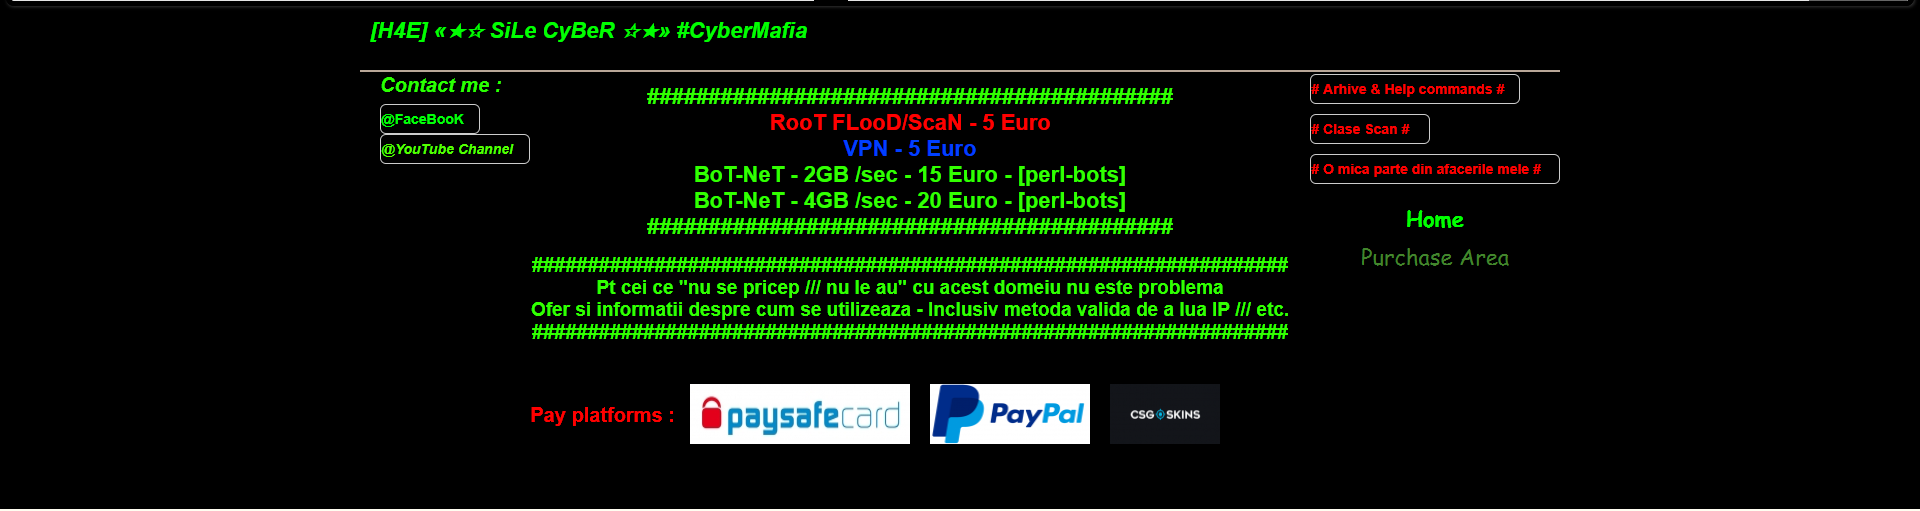
\includegraphics[width=160mm, scale=1]{Images/cybermafia_ddos-for-hire.PNG}
      \caption{DDoS-for-Hire: The Web Domain of a Human Attacker} 
      \medskip
      \small
		The webpage shown was linked to an attack session in the router container honeypot, where a Python script was downloaded from this site and used to measure the network bandwidth available to the system. The homepage shown in this image advertises DDoS-for-hire services, where it costs  \euro{15} to buy a 2GB/second attack and a 4GB/second attack costs \euro{20}.
\label{fig:CyberMafiaDDoSForHire}
\end{figure}
 
%\includewidefigure{CyberMafiaDDoSForHire}{DDoS-for-Hire: The Web Domain of a Human Attacker}{The webpage shown was linked to an attack session in the router container honeypot, where a Python script was downloaded from this site and used to measure the network bandwidth available to the system. The homepage shown in this image advertises DDoS-for-hire services, where it costs  \euro{15} to buy a 2GB/second attack and a 4GB/second attack costs \euro{20}.}{Images/cybermafia_ddos-for-hire.PNG}


\subsection{Concluding the Honeypot Experiments}
Something that became very clear from the experiments conducted was the unpredictability of conducting honeypot experiments. Given that 4 weeks had been allocated to complete all 12 iterations of experiments planned, it was crucial that there were minimal setbacks to the progression of the experiments within this time.

Over a week after setting up the first of these 12 iterations, the first experiment iteration had been deployed a total of three times due to the issues outlined in \textit{Section \ref{ConductingExperiments}}. It was concluded that conducting the remainder of the planned experiments was infeasible, given that less than three weeks remained to conduct the remaining iterations. Thus, the conducting of the planned experiments was discontinued.



%
%	SECTION 3: DISCUSSION
%


\section{Discussion} \label{DiscussionOfEvaluation}
% Will be more qualitative than quantitative.
Both the achievements and the limitations of the research are evaluated and discussed in this section. 

\subsection{Honeypot-Driven Cyber Incident Monitoring}
The first objective of this research was to develop a honeypot-driven cyber incident monitor that would be feasible to deploy in modern IT infrastructures, making it feasible for organisations to implement active network defence.

\subsubsection{Effectiveness of  the Containerised Honeynet}
% Piscarcik refer to the same paper:  scalability, flexibility, compromise, non-detectability and ease of deployment are key requirements for such a system.
As one of the novel features of the implemented incident monitoring system, the effectiveness of the honeynet deployment proposed by this research forms an important component of the evaluation. A useful set of criteria outlined by Chin \textit{et al.} \cite{5319295} and used by Piscarcik \textit{et al.} \cite{Pisarcik:2014:FDV:2659651.2659685} to evaluate their honeynet deployments specifies a number of key criteria that should be fulfilled by an effective honeynet. These are discussed below in relation to the system implemented in this research.

\begin{enumerate}
\item \textbf{Scalability}

The proposed solution is scalable insofar as it has been tested. The largest honeynet deployment trialled during the research consisted of 11 containerised honeypots\footnote{10 Cowrie honeypot containers and the router honeypot container.}, which was hosted continuously for 2 days without any component failing. However, during this period there was very little interaction with the system, limiting the load on system resources that would be present in a production environment.

In theory, the honeynet is capable of supporting a large number of honeypot containers. The ability to add more honeypots is largely dependent on the system resources available: The host system must have sufficient resources to support the number of containers  deployed. This is however certain to be much less than that required for an equivalent number of virtual machines on the same host.
 
\item \textbf{Flexibility} 

The implemented honeynet solution is flexible in its operability, configurability and maintainability. 
\begin{itemize}
\item Control over the honeynet from an administrative perspective is straight-forward: Containers can be managed through the host even whilst running, meaning that reconfiguration of the networking and administrative access to container resources can be done on-the-fly as required.
\item The use of the Cowrie honeypot also contributes to the flexibility of the honeynet. As a highly configurable and customisable open-source honeypot, tweaking the configuration of the honeypots in response to new threat insights is very achievable. 
\item It would also be relatively straight-forward to use a different honeypot in place of Cowrie in this system: Without having to make any changes to the network configuration, new Dockerfiles can be defined for alternative honeypots if required, integrated to the system with simple edits to the deployment script.

\end{itemize}
\item \textbf{Attack Containment}

Attack containment refers to the restriction of propagation of attacks if a honeypot is compromised. Though attack containment is never completely assured, the measures taken to provide attack containment described in \textit{Section \ref{DockerSecurityConsiderations}} mitigate against undesirable attack propagation outside the honeynet.
\begin{itemize}
\item The isolation of the host from the \textit{dmz} network on which the honeynet is hosted restricts the ability of an attacker to launch a network-based attack from within the honeynet. 
\item The carefully considered restrictions placed on an attacker inside the Cowrie honeypots mean that it is highly improbable that an attacker would be able to launch an attack from these honeypots in the first place. The fact that the Cowrie honeypot is an emulated environment in particular restricts an attackers activities, since they are not interacting with a real system with a networking stack, OS and powerful utilities.
\item The high-interaction router container is the only component of the system where attack containment may not be fully assured, since this container interfaces directly with a network to which the host is connected. This is a potential area for improvement, where given additional time investigating the use of alternative networks that don't interface with the host system could yield an improved level of isolation.
\end{itemize}
\item \textbf{Stealth}

Stealth refers to the ability of the honeynet to deceive an attacker and convince them that it is a legitimate system. It is difficult to provide a definitive conclusion regarding this property of the deployed honeynet, given that the interactions of attackers with the system were limited at best. 

There is certainly scope for improvement of the stealth of the honeynet based on the little data that was obtained through the experiments outlined in \textit{Section \ref{ConductingExperiments}}, since in each iteration it was found that IoT bot attackers did not progress their attacks beyond their known initial phases. \cite{UnderstandingTheMiraiBotnet} \cite{HajimeMysteriousBotnet}  To reach any definitive conclusions about this property would require substantially more time and experimentation.

However, the properties of the containerised honeynet lend themselves to deceiving attackers about the legitimacy of the environment, since all honeypots are hosted in containers with real OS images and networking stacks. For instance, Chin \textit{et al.} propose that stealth can be achieved through measures such as falsifying high network latency. \cite{5319295} An attacker testing the legitimacy of this honeynet based on such properties will receive legitimately delayed responses by virtue of the use of containers in the system.

\item \textbf{Resource Management} 

This criterion refers to the presence of simple mechanisms for allocating resources in the honeynet, which is largely provided through the use of Docker in this implementation. 
\begin{itemize}
\item The nature of containers is that the resources allocated to the running of an application are highly controlled and specified entirely by their image definition. In order to allocate additional resources, a simple update to this image definition is all that is required.
\item The host system resources consumed by containers are controllable primarily through the specification of arguments when creating containers. As stated in the Docker documentation, ''by default, a container has no resource constraints ... Docker provides ways to control how much memory, CPU, or block IO a container can use, setting runtime configuration flags of the docker run command''. \cite{DockerResourceConstraints} Though these resource restrictions were not explicitly addressed as part of the development of the containerised honeynet, it would be straight-forward to add these resource restrictions to the deployment script as part of  the \textit{docker create} commands.
\end{itemize}


\item \textbf{Ease of Deployment} 

Chin \textit{et al.} state that for a honeynet to be considered easy to deploy, ''users are not burdened by complicated configurations and procedures in order to set up their own honeypots''. 

In the proposed system, the use of containers and the automation of network configuration through scripting means that a fully configured honeynet of connected containers can be removed and re-deployed on a Linux host in approximately 5 minutes\footnote{This value is based on empirical timing measurement of the time taken to deploy the system from scratch on a clean EC2 host.}. As the initial motivation behind using containers in the proposed system, this criterion has certainly been met by the system.

Ease of usability through an interface to the system is also highlighted by Chin \textit{et al.} as being of importance to the ease of deployment of a honeynet. \cite{5319295} The usability aids implemented in the \textit{do\_honeypot.sh} deployment script remove additional complexity from the deployment process, providing simple console messages to guide in the deployment and configuration of the system.
\end{enumerate}
Thus, it is concluded that although there is room for improvement of various aspects of the implemented honeynet, the requirements outlined in this classification have largely been delivered by this system.


\subsubsection{Architecture of the Monitoring System}
\label{CentralisedManagementEvaluation}
A limitation that has been identified upon evaluation of the system architecture is that of the centralisation of log processing in the incident monitor. Although the centralised aggregation of honeypot data for visualisation in the system enables the correlation of attack data to provide a holistic view of the entire honeynet, it also means that the system is architected in such a way that it has a single point of failure.

The current system architecture is non-ideal from the perspective of system reliability, since if the EC2 management server instance was to become overloaded and crash, the incident monitoring system would no longer be able to provide its intended service. A more distributed approach to processing and visualising data generated by the honeynet would improve the reliability of the proposed system. This will be discussed in \textit{Section \ref{AlternativeSystemArchitectureFW}} in the context of future work for this project.

However, there are some features of the architecture of the implemented system which make it more scalable: In particular, that the honeynet in this deployment is hosted locally with Docker rather than as a distributed network. In the evaluation of the \textit{TraCINg} incident monitor by Vasilomanolakis \textit{et al.} \cite{Vasilomanolakis}, they note that their distributed architecture creates a bottleneck with regards to resource competition ''when the number of new sensors is massively increased'', since multiple distributed honeypots individually provide their results to the centralised incident monitoring system. In the system developed in this research, the data generated by the honeypots is aggregated locally through the use of Docker volumes and CRON rather than being transmitted by each honeypot, reducing the network traffic to the centralised management instance.

\subsubsection{Impact of Visualisation on the Usability of Honeypots}
The use of visualisation in this project was motivated by the need to make honeypot-driven solutions more usable, providing a way for administrators to easily obtain a holistic view of the state of active network defence in their systems.

Though there was no experimental data captured by the Cowrie honeypots whose logs could be processed and visualised on the Kibana web interface, simulated attacks were conducted to allow visualisations to be produced for evaluation. Figures \ref{fig:Some_Cowrie_visualisations_on_the_Kibana_dashboard_.PNG}, \ref{fig:Cowrie_Attacks_per_honeypot.PNG} and \ref{fig:Cowrie_most_popular_protocol_per_honeypot_this_month.PNG} illustrate the capacity of the ELK log management stack to communicate complex log data concisely and effectively.

\begin{figure}[ht]
      \centering
      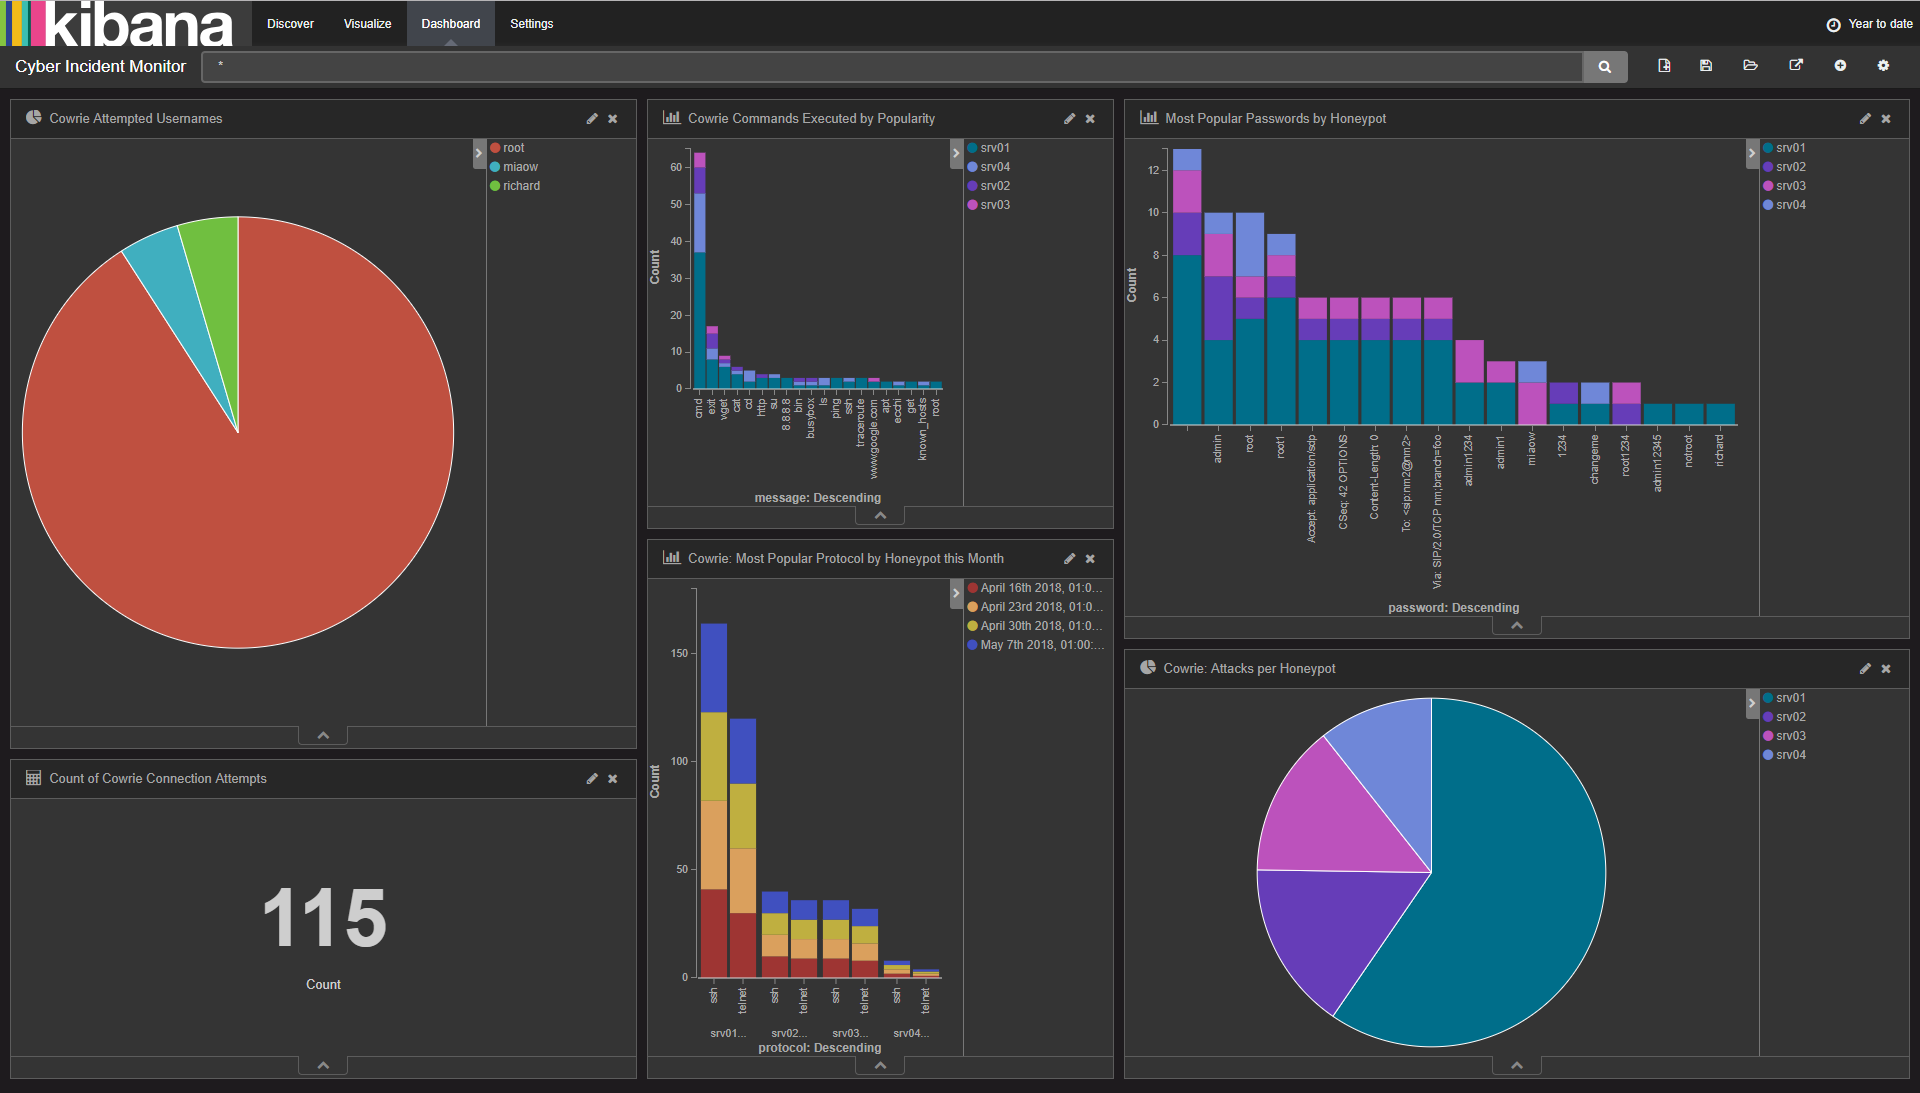
\includegraphics[width=160mm, scale=1]{Images/Some_Cowrie_visualisations_on_the_Kibana_dashboard_.PNG}
      \caption{Cyber Incident Monitor on Kibana} 
      \medskip
      \small
		This image shows the Kibana visualisation dashboard that was created as part of the incident monitoring solution. A number of charts are shown, measuring everything from the popularity of passwords per honeypot to the proportion of telnet and SSH attacks received by each Cowrie honeypot. The dashboard provides a concise description of the threat state of the honeynet.
\label{fig:Some_Cowrie_visualisations_on_the_Kibana_dashboard_.PNG}
\end{figure}

%\includewidefigure{Some_Cowrie_visualisations_on_the_Kibana_dashboard_.PNG}{Cyber Incident Monitor on Kibana}{A collection of visualisation created in Kibana for the cyber-incident monitor.}{Images/Some_Cowrie_visualisations_on_the_Kibana_dashboard_.PNG}

\begin{figure}[ht]
      \centering
      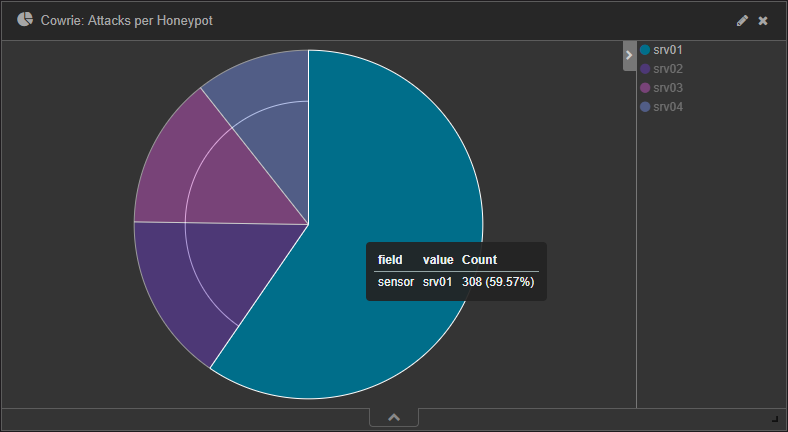
\includegraphics[width=160mm, scale=1]{Images/Cowrie_Attacks_per_honeypot.PNG}
      \caption{Visualisation: Attacks per Honeypot} 
      \medskip
      \small
		This image shows a single visualisation created in Kibana as part of the cyber-incident monitor. This pie-chart shows the proportion of attacks each Cowrie honeypot received within a month.
\label{fig:Cowrie_Attacks_per_honeypot.PNG}
\end{figure}

%\includewidefigure{Cowrie_Attacks_per_honeypot.PNG}{Visualisation: Attacks per Honeypot}{A visualisation created in Kibana as part of the cyber-incident monitor. This pie-chart shows the proportionately how many attacks each honeypot received within a week.}{Images/Cowrie_Attacks_per_honeypot.PNG}

\begin{figure}[ht]
      \centering
      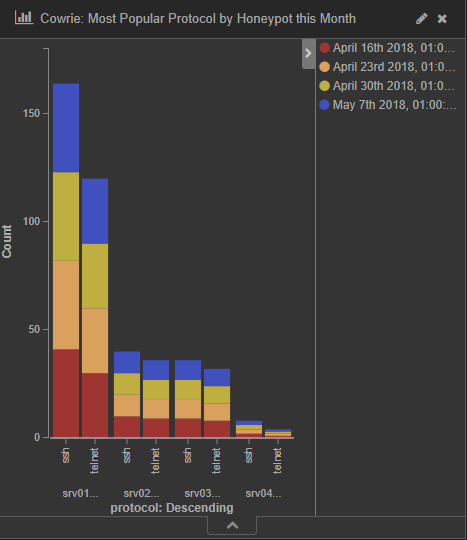
\includegraphics[width=100mm, scale=0.2]{Images/Cowrie_most_popular_protocol_per_honeypot_this_month.PNG}
      \caption{Visualisation: Most Popular Protocols per Honeypot by Month} 
      \medskip
      \small
		This image shows another visualisation created in Kibana as part of the cyber-incident monitor. This chart shows the proportion of SSH and Telnet attacks received by each of the honeypots for each week over the last month.
\label{fig:Cowrie_most_popular_protocol_per_honeypot_this_month.PNG}
\end{figure}

%\includewidefigure{Cowrie_most_popular_protocol_per_honeypot_this_month.PNG}{Visualisation: Most Popular Protocols per Honeypot by Month}{A visualisation created in Kibana as part of the cyber-incident monitor. This chart shows the proportion of SSH and Telnet attacks received by each of the honeypots for each week over the last month.}{Images/Cowrie_most_popular_protocol_per_honeypot_this_month.PNG}

What can be noted about these visualisations is the effectiveness with which information is imparted to the user: Rather than sifting through reams of honeypot log data, correlated information regarding attack behaviours and patterns is represented succinctly in the visualisations. The fact that the logs used to produce these are shipped from the honeypot server approximately every 60 seconds\footnote{As explained in \textit{Section \ref{CRON}}, the honeypot logs were made available to Filebeat every 60 seconds before being shipped to the EC2 management instance. Any additional delay in delivery is likely to be due to network conditions.} means that an administrator is facilitated in understanding the current threats to their system rapidly. 





\subsection{The Design of Adaptive Honeypots}
As such, it would appear that unpredictability is the nature of research where honeypots are involved. It had been hoped that a quantitative evaluation would be provided in this section: However, due to the issues encountered with completing all planned iterations of experiments, the evaluation of the contribution of this research towards the design of adaptive honeypots is restricted by the incomplete results obtained in \textit{Section \ref{ConductingExperiments}}.

\subsubsection{Unpredictability of Honeypot Experiments}
It has been found that the process of designing honeypots to be adaptive to dynamic threats is a time-intensive one. Unforeseen issues such as the requirement to implement a high-interaction container honeypot, and the further significant challenges which were faced in implementing this effectively, are illustrative of the unpredictability of designing adaptive honeypots. 

The fact that the contributions of just 3 characteristics of honeypots were considered in the experiments outlined in \textit{Section \ref{DesignOfExperiments}} is explained by the limited remaining time within which the experiments could be conducted. Had more time been available, a set of comprehensive honeypot experiments could be conducted accounting for several other honeypot characteristics. 

When compared to the time spent conducting similar research experiments in the closely related projects discussed in \textit{Section \ref{CloselyRelatedWork}}, the findings were as follows:
\begin{itemize}
\item The researchers involved in the \textit{IoTPot} project conducted experiments to evaluate the effectiveness of their design in 2 separate phases: a 144-day trial period from 2014/11/07 to 2015/03/31 which was used to ''understand the attackers' behavior and (discuss) the proper setting of the honeypots'', followed by a 28-day stable period from 2015/04/01 to 2015/05/09 in which more structured experiments were conducted. \cite{IoTPot2016}
\item In their evaluation of honeypot performance in the \textit{TraCINg} incident monitor, Vasilomanolakis \textit{et al.} explain that a five-month deployment of their honeypot-driven incident monitor allowed them to obtain meaningful results.  \cite{Vasilomanolakis}
\end{itemize}
These findings further illustrate the unpredictability of evaluating the effectiveness of honeypots. It is perhaps an oversight that the time that would be required to conduct such experiments was not realised at an earlier stage.

In recognition of the fact that none of the experiments conducted could provide \textit{conclusive} evidence regarding the design of adaptive honeypots, there was a need to consider what was (i) necessary, (ii) sufficient and (iii) additional towards the achievement of the original objective.

\begin{enumerate}
\item \textbf{Necessary}

It is necessary that knowledge is gained about the contribution of a honeypot's design to its effectiveness in attracting attacks through experiments. 
\item \textbf{Sufficient}

It is sufficient that the knowledge gained is not conclusive but is based on experimental data.

\item \textbf{Additional}

It is additional that the knowledge gained is definitive and conclusive based on experimental data.

\end{enumerate}
It is clear that obtaining conclusive results regarding effective design for adaptive honeypots  became infeasible because of time constraints, ultimately resulting in the early termination of the experiment phase. However, the data obtained from the three experiment attempts, although not definitive, did provide some insights into the nature of designing adaptive honeypots.
\begin{itemize}
\item The presence of expected utilities and toolkits in a honeypot environment is clearly crucial to its success in encouraging attacks. This was evident from the data captured in attempts 2 and 3 of the experiment iteration performed, where bot attackers did not proceed with compromise of the system when certain utilities were not present in the honeypot environment.
\item Support for protocols and services which are commonly exploited by attackers is an important feature of effective honeypots: this is evident by virtue of the sheer volume of brute-force authentication attacks which were received
\item Basing honeypot design on current knowledge of attacks is a useful starting point in enabling attacks to be studied. In the design of the high-interaction router honeypot, it is likely that the experiments would have been more successful if more emphasis had been placed on configuring the environment to provide responses and utilities sought after by active IoT botnets, knowledge of which already exists in research. \cite{UnderstandingTheMiraiBotnet} \cite{HajimeMysteriousBotnet}
\item Honeypots must be designed to combat both automated and human attackers. It was not expected based on the findings of Barron \textit{et al.} that attacks by human attackers would be likely to be encountered in the honeypot environment. \cite{PickyAttackers2017} The fact an attack session by a human attacker was captured in the limited period for which experiments were conducted illustrates that honeypots should be designed to adapt to threats from human attackers, and not solely the more predictable attack patterns of bots. 
\end{itemize}
\subsubsection{Ability to Capture Attack Data}
As evidenced during the conducting of experiments in \textit{Section \ref{ConductingExperiments}}, the fact that keylogging was not available on the router container honeypot severely limits the conclusions that can be drawn regarding any experimental results that were obtained. For instance, although patterns of command execution were observed in the \textit{.bash\_history}, the lack of timestamping and session IDs for these events meant that inferences were made regarding these sequences being from a single attacker. 

There is plenty of room for improvement regarding the capturing of attack data, and given more time, it would almost certainly be possible to develop an effective and reliable keylogging mechanism for the router container. 

\subsubsection{Hosting Honeypot Experiments on a Cloud Platform}
It is quite probable that some of the attack patterns observed in \textit{Section \ref{ConductingExperiments}} may have been different had a different hosting solution been used to host the system. As noted by Vasilomanolakis \textit{et al.} in their implementation of a honeypot incident monitor, \cite{Vasilomanolakis} many cloud service providers publish their IP ranges on the public internet: AWS is one such provider. \cite{AWS_PublicIPRanges} In their paper examining the difference between human and automated attacks, Barron \textit{et al.}  also find that ''location and host matters... if someone is operating on a constrained budget and wants to maximize the number of brute-forcing IP addresses collected, AWS appears to be the infrastructure that will facilitate this''. \cite{PickyAttackers2017}

As AWS are a very well-known and popular cloud hosting provider, they are likely an attractive target for attackers who have knowledge of their public IP ranges. Thus, there is potential for some bias in results obtained in a deployment such as that implemented in this research, where all honeypots are hosted in a single geographical region by a single hosting provider. 
 
%Allowing IoT bot attackers to authenticate easily is important, so supporting as many username-password combinations as possible is a good idea. This is in line with what was found by the IoTPot researchers. \cite{IoTPot2016}
%Providing the utilities that the attacker expects to find is also important, since it was ultimately issues like this that resulted in repeating the first experiment.
%High-interaction IoT honeypots take a lot of maintenance


\subsubsection{Fingerprinting Container Environments}
An interesting observation regarding the fingerprinting of honeypot environments is that there are many ways in which an attacker can detect that they are inside a container, if the honeypot is indeed the container itself. This was noted during the implementation of the system, when the command \textit{cat /proc/1/cgroup} was executed, leading to the output shown in figure \ref{fig:DockerFingerprintingCommand}. This is consistent with the findings of Kedrowitsch \textit{et al.} when evaluating the suspectibility of containers to being fingerprinted. \cite{LXCsForDeceptiveHoneypots2017}

\begin{figure}[ht]
      \centering
      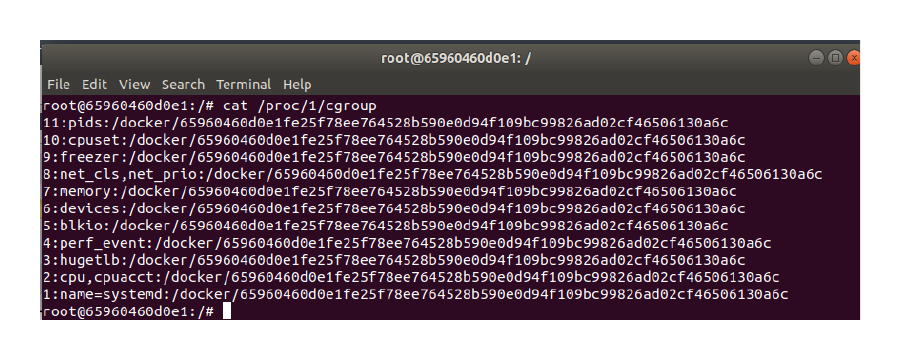
\includegraphics[width=160mm, scale=1]{Images/Fingerprinting_Docker_Containers__1_.png}
      \caption{Fingerprinting of Docker Environments} 
      \medskip
      \small
		This console output was generated as a result of executing the command \textit{cat /proc/1/cgroup} inside the router container. It clearly includes several references to 'docker', which any attacker aware of Docker would immediately recognise as being a container environment.
\label{fig:DockerFingerprintingCommand}
\end{figure}

%\includewidefigure{DockerFingerprintingCommand}{Fingerprinting of Docker Environments}{This console output was generated as a result of executing the command \textit{cat /proc/1/cgroup}. It clearly includes several references to 'docker', which any attacker aware of Docker would immediately recognise as being a container environment.}{Images/Fingerprinting_Docker_Containers__1_.png}

This may not come as a surprise to an attacker: As organisations increasingly include containers as part of their infrastructure, this information would likely not identify the container as being a honeypot. However, it is certainly worth considering that if containerised honeypots begin to be used more widely, fingerprinting of these systems as honeypot environments may also become more common. 


\section{Summary} \label{SummaryOfChapter6}

It is clear that the unpredictability of conducting honeypot experiments was a barrier to obtaining measurable data and providing definitive conclusions regarding the adaptive design of honeypots. This was largely an oversight in the design phase of the research, where had more time been available, there would have been a greater opportunity to achieve this objective as part of this research.

However inconclusive, useful insights have been obtained from the experiments conducted. This is an encouraging indication of the potential for a real contribution to be made through experiments of this nature, and provides a strong basis for completing the remaining iterations of the project as future work.